\chapter{Methodology}\label{methodology}
    This chapter provides an overview of our designed procedures and algorithms. As mentioned in the earlier in the thesis objectives, the goal is to design and implement a framework that tracks people in the video sequence followed by additional information extraction on person-specific features. Before getting into our the tracker design, we present our data acquisition and data pre-processing process. Later then, we propose a people detector and tracker which follows the well-known tracking-by-detection approach and in the end, we present strategies for additional information extraction. 

\section{Image acquisition}
    Image acquisition is the first stage in any vision processing system. The goal of image acquisition is to transform real-world optical data into an array of numbers that can be processed by a computer. The process heavily depends on the camera and lens hardware. 
    
    The main component of the camera is its sensor that converts light into electrical charges, while the lens focuses the light on particular spots of the sensor. Nowadays, the most used technology for the camera sensor is \gls{cmos} due to its low noise and processing speed capabilities. Since the work is done in cooperation with well-equipped \gls{improlab} at \gls{fit} \gls{ctu}, we have a choice of several camera and lens variants available.
    
    Based on assumptions and thesis instructions, we know the scene, and its parameters in advance. To test the designed algorithms of this work, we chose the scene to be the 14th floor of the \gls{fce} \gls{ctu} building near elevators. Based on the scene, we selected the appropriate combination of lens and camera sensitive to the visible spectrum. The \gls{improlab} has most of its cameras from Basler manufacturer. Thus we decided to utilize Basler ace acA1920-50gc \cite{baslercamera}, the \gls{gige} camera with the Sony IMX174 \gls{cmos} sensor that delivers 50 \gls{fps} at 2.3 \gls{mp} resolution. Due to the spatial properties of the scene, we chose Basler 8mm lens C125-0818-5M F1.8 \cite{baslerlens} that proved to be the best option in this case.
   
    \begin{figure}[h]
        \centering
        \subfloat[]{{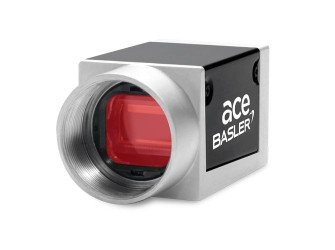
\includegraphics[width=0.35\textwidth]{resources/basler_camera.jpg} }}
        \qquad
        \subfloat[]{{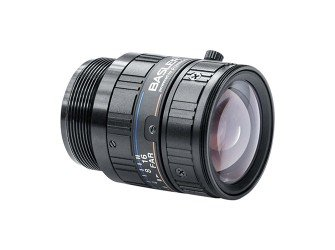
\includegraphics[width=0.35\textwidth]{resources/basler_lens.jpg} }}
        \caption{Selected camera equipment for our task. a) Camera Basler ace acA1920-50gc. b) Lens Basler 8mm  C125-0818-5M F1.8. Source: \cite{baslercamera, baslerlens}}.
        \label{fig:camera_equipment}
    \end{figure}
    
    The image stream from Basler's camera equipment can be obtained in several ways. The most convenient but limiting approach is to use Basler pylon Camera Software Suite, which is a software package comprised of an easy-to-use \gls{sdk}, drivers and tools that can be used to operate any Basler camera using the user interface on multiple platforms such as Windows, Linux, and Mac. However, this option does not allow integration with custom software. Another option is to use Basler's pypylon \cite{baslerpypylon} which is the new open source wrapper interface for the Basler pylon Camera Software Suite that allows direct camera access through Python code.
    
    Due to the nature of the work, the data can be in an offline form. Thus we decided to use the first method with the Basler pylon framework because it is more convenient than the pypylon wrapper.
    
    We record the video sequence at the highest possible resolution, i.e., 1920x1080 and at 25 \gls{fps}. Each frame is saved in a jpg format to avoid an overhead that would be caused by decoding the video formats. The camera shutter speed is set manually so that people in the scene are not motion blurred and the aperture is set to the sweet-spot of the lens, which in our case is f/4.0, to achieve maximum image quality. Since these parameters would make the image too dark, it is necessary to increase the sensor gain value. In this case, we decided to set sensitivity value to automatic, which means that it is always calculated so that the scene is exposed correctly.  We set the white balance to a fixed value determined by automatic detection to avoid drastic color changes during shooting. We provide an example of the scene in Fig. \ref{fig:scene_example}.

    \begin{figure}[ht]
        \centering
        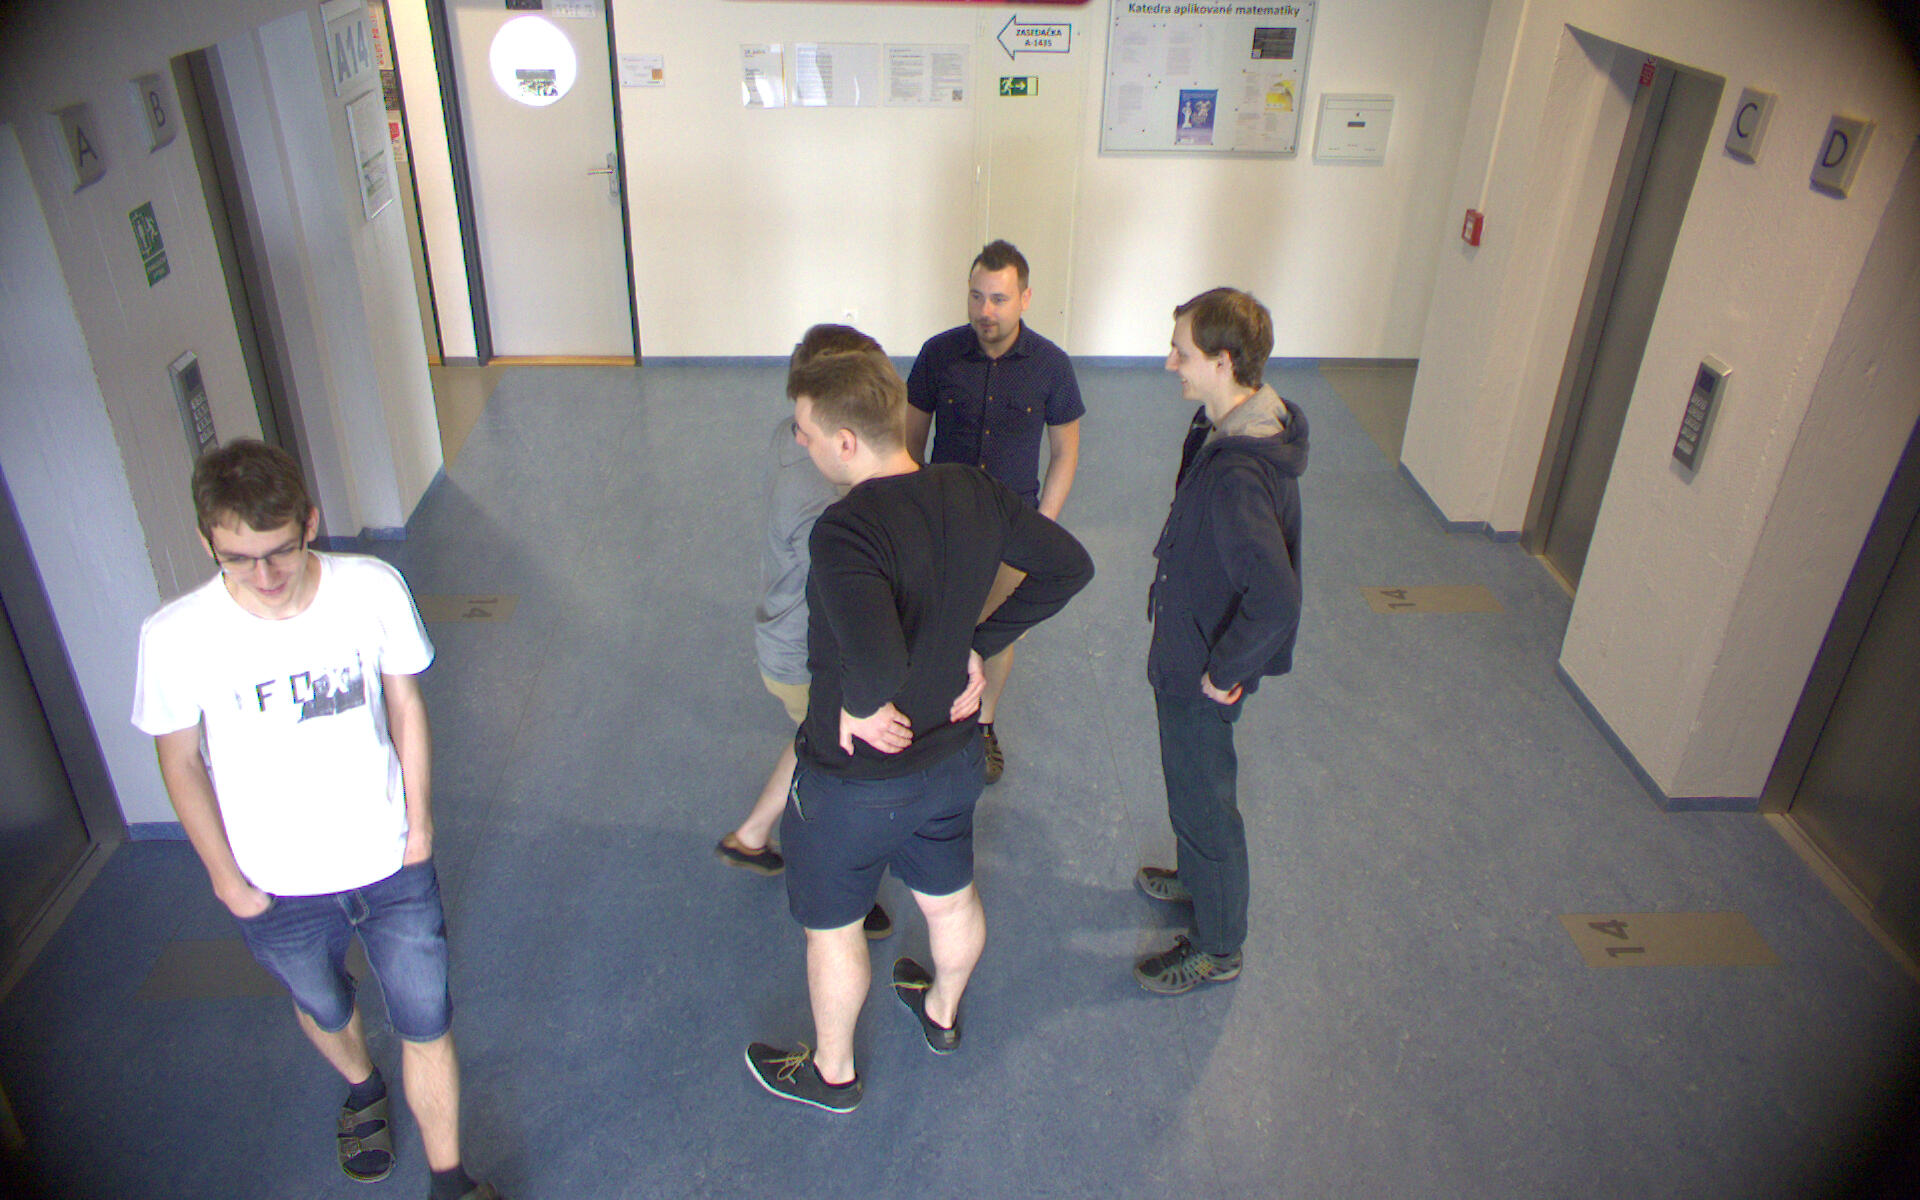
\includegraphics[width=0.75\textwidth]{resources/scene_example.png}
        \caption{Example of the acquired image and the scene layout. We can see that despite being a quality lens, it contains distortion and vignetting.}
        \label{fig:scene_example}
    \end{figure}
        

\section{Image pre-processing}
    After the images are obtained, various pre-processing methods can be applied to improve the accuracy of feature extraction and classification methods. However, in our case, we assume that all images are acquired in satisfactory quality and with proper exposure, shutter speed, and white balance settings. The only pre-processing we do is removing lens distortion by using a camera calibration method as described in \ref{camera_calibration}.

\section{Detection and tracking components}\label{detection_and_tracking_components}
    In this section, we present our design decisions for two core components of our framework -- the detector and the tracker. In contrast to batch based approaches, we primarily target online tracking where only information from the previous and current frame is available. We also try to maintain both components as much as efficient as possible for further extension to real-time applications.

    The \gls{mot} can be viewed as a data association problem, where the goal is to associate hypotheses obtained from the object detector across frames in a video sequence. One way to solve this problem is to compare and match specific features such as the appearance and motion of objects in the scene. 
    
    The methods employed in the tracker are inspired by work \cite{2016arXiv160502688short}, that performs Kalman filtering \cite{kalman1960new} in image space and frame-by-frame data association using the Hungarian method \cite{jonker1987shortest} with an association metric that measures bounding box overlap, and by \cite{wojke2017simple} that improves the previous approach by adding deep association metric.

    \subsection{People detection}
        The beginning of the tracking process is an object detection step. In this work, we use various detector models based on \gls{yolo} and \gls{faster r-cnn} with ResNet50 backbone. The result of forwarding the frame through \gls{cnn} architecture is in the form of hypotheses that contains bounding box coordinates, object class, and detection confidence. Except for input image resizing to be compatible with the \gls{cnn}, we do not perform any other pre-processing in this phase.
        
        Object detectors are usually trained on multiple object classes, but as we are only interested in people, we filter out all other classes from the output hypotheses. We also filter out low-confidence ones. The confidence threshold is variably configured according to the object detector used. \Gls{faster r-cnn} produces a lot of false positives. Thus we take into account only hypotheses with confidence greater than 90 \%. In \gls{yolo}, the threshold value of 70~\% has been experimentally verified to work well. We employ both network architectures with their default parameters trained on the COCO dataset \cite{lin2014microsoft}. 
        A common problem of object detectors is that they often generate more overlapping hypotheses than the ground-truth objects (false positives). To handle the removal of overlapping bounding boxes we use additional \gls{nms} step \cite{rosebrocknms} for bounding box post-processing.
        
        \begin{figure}[ht]
            \centering
            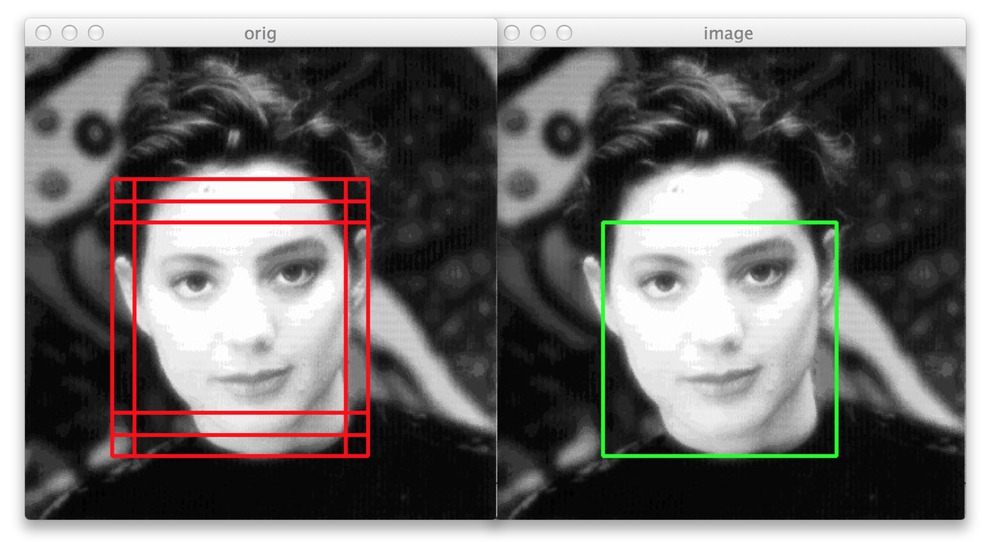
\includegraphics[width=0.75\textwidth]{resources/non_maximum_surpression.png}
            \caption{Six bounding boxes are detected around the face, but by applying non-maximum suppression, it is possible to remove the redundant ones. Source: \cite{rosebrocknms}.}
            \label{fig:non_maximum_surpression}
        \end{figure}
        
    \subsection{Track handling}
        To maintain object identities and propagate object states into the future, we need to maintain historical information in the memory about previous detections. To achieve this goal, we define track object class, and in each frame, we associate current detections with existing track objects (tracks). While the detected hypothesis is only represented by an object class, bounding box and confidence, a track contains multiple attributes such as identity, status, time since the last update, age in frame units, bounding box, state, and class-specific information.
        
        When a person enters or leaves the scene, unique identity needs to be created or removed accordingly. For initiating a new track, we take detections that were not successfully associated in the matching phase of the current frame (unmatched detections). These fresh tracks are then set to tentative during their first $t_c$ frames. Tracks that are not successfully associated during the $t_c$ frames are removed from the scene, which helps to accumulate enough evidence to prevent tracking of false targets. Each track also has a variable that determines the number of frames of the last successful association. Tracks are terminated if they are not associated within $t_m$ frames or their state predictions are outside of the frame. Based on our experiments we have selected a value $t_c = 7$ for track confirmation and $t_m = 50$ for track termination. Due to camera settings, the termination based on our value of $t_m$ means that the appropriate detection was not found for two seconds. 
        
    \subsection{State estimation}
        The state representation helps to propagate a track's identity into the next frames. The inter-frame displacements of each track are approximated with a linear constant velocity model which is independent of other objects. Our design of the track's state is represented as a 10-dimensional vector:
        
        \begin{equation}\label{state_vector}
            x = \left(cx, cy, ty, h, r, \dot{cx}, \dot{cy}, \dot{ty}, \dot{h}, \dot{r} \right), 
        \end{equation}
        
        where $cx$, $cy$ represent center pixel location of the bounding box, $ty$ represent the top center location of the bounding box, $h$ is pixel height, and $r$ is the aspect ratio of the bounding box. Each of these parameters has its respective velocities in image coordinates. 
        
        To predict and estimate the accurate value of track states, we use standard Kalman filter \cite{kalman1960new}. It is a recursive algorithm with a real-time performance that is commonly used to extract the useful signal from noisy measurements. In this case, it can be used to refine the bounding box position. 
        
        The whole filtering process consists of two main steps -- prediction and correction. In the prediction phase, the filter produces predictions of the current state variables, along with their uncertainties. Furthermore, once the output of the next measurement is known, it is used in a correction step to update state variables with a weighted average. The weights are greater for values with higher certainty.
  
        The Kalman filter assumes that the real state at time $k$ can be obtained from state $k - 1$ by the following prediction equation: 
        
        \begin{equation}
            x_k = F_k x_{k-1} + B_k u_k + w_k,
        \end{equation}
        
        where $F_k$ is the  state-transition model, $B_k$ is the control-input model applied to the control vector $u_k$, $w_k$ is the process noise, assumed to be drawn from 
        $w_k \sim {\mathcal {N}} (0,Q_k)$, and $Q_k$ is covariance matrix with appropriate dimensions.
        
        Measurements $z_k$ at time $k$ then can be obtained as follows:
        
        \begin{equation}
           z_{k} = H_{k} x_{k} + v_{k},
        \end{equation}
        
        where $H_k$ is the observation model which maps the true state space into the observed space, $v_k$ is the observation noise, assumed to be drawn from 
        $v_k \sim {\mathcal {N}} (0,R_k)$, and $R_k$ is covariance matrix with appropriate dimensions. All filter parameters are supposed to be correctly user-defined. Otherwise, the filter will not have the required properties.

        In our design, we do not assume the variability of matrices $F_k, Q_k, H_k, R_k$ in time and we can drop $B_k$ since we do not have any control input. $F$ is then designed according to state vector (defined in \ref{state_vector}) and constant velocity model as follows:
        \begin{equation}
            F = 
            \begin{pmatrix}
                1 & 0 & 0 & 0 & 0 & dt & 0 & 0 & 0 & 0 \\
                0 & 1 & 0 & 0 & 0 & 0 & dt & 0 & 0 & 0 \\
                0 & 0 & 1 & 0 & 0 & 0 & 0 & dt & 0 & 0 \\
                0 & 0 & 0 & 1 & 0 & 0 & 0 & 0 & dt & 0 \\
                0 & 0 & 0 & 0 & 1 & 0 & 0 & 0 & 0 & dt \\
                0 & 0 & 0 & 0 & 0 & 1 & 0 & 0 & 0 & 0 \\
                0 & 0 & 0 & 0 & 0 & 0 & 1 & 0 & 0 & 0 \\
                0 & 0 & 0 & 0 & 0 & 0 & 0 & 1 & 0 & 0 \\
                0 & 0 & 0 & 0 & 0 & 0 & 0 & 0 & 1 & 0 \\
                0 & 0 & 0 & 0 & 0 & 0 & 0 & 0 & 0 & 1 \\
            \end{pmatrix},
        \end{equation}
        where $dt$ is chosen to be 1. Matrix $H$ for obtaining measurements is given by:
       \begin{equation}
            H = 
            \begin{pmatrix}
                1 & 0 & 0 & 0 & 0 & 0 & 0 & 0 & 0 & 0 \\
                0 & 1 & 0 & 0 & 0 & 0 & 0 & 0 & 0 & 0 \\
                0 & 0 & 1 & 0 & 0 & 0 & 0 & 0 & 0 & 0 \\
                0 & 0 & 0 & 1 & 0 & 0 & 0 & 0 & 0 & 0 \\
                0 & 0 & 0 & 0 & 1 & 0 & 0 & 0 & 0 & 0 \\
            \end{pmatrix}.
        \end{equation}
        The noise matrices are heavily dependant on the captured scene, but generally speaking, we set significantly higher variance values in for measurement noise matrix $R$ then process noise matrix $Q$. This is because an object detector produces sparse detections with noisy bounding box predictions.

        To sum it up, each track has its state as defined in \ref{state_vector}. When detection is associated with a track, the bounding box coordinates are used as a measurement to update the internal state of the filter. Velocity components are then solved optimally via the filter's transition matrix. If detection is not associated with a track, its state is predicted using a linear model (skipping the correction step). 
        
        More details on the filter assumptions, properties and calculations can be found in its original proposal \cite{kalman1960new}.

    \subsection{Appearance features}\label{appearance_features}
        Using only state estimation in the matching phase would result in a high number of identity switches due to occlusion effects and non-linearity in people's behavior. Therefore, appearance descriptors are often extracted to make hypothesis-to-track matching more robust. At the beginning of this work, we tried to use color histograms of bounding box patches as appearance descriptor. Patches were then converted to \gls{hsv} color space to make them comparable by Bhattacharyya distance \cite{choi2003feature} with hue and value channel as input. However, object histograms are greatly affected by their background. Thus this solution was not robust, and we decided not to continue this path.
        
        Instead, we utilized a \gls{cnn} model from \cite{wojke2017simple} that has been trained to discriminate pedestrians on a large-scale dataset. The input of the model is a bounding box patch of a person and based on that it outputs 128-dimensional vector comparable with cosine distance metric. Through the integration of this feature descriptor, it is possible to recover track's identities even in long-term occlusions.

    \subsection{Data association}
        To create associations between existing tracks and newly arrived detections it is convenient to solve the assignment problem using the Hungarian algorithm \cite{jonker1987shortest}. The values of cost matrix are calculated through a combination of two appropriate metrics -- state and appearance. 
        
        \subsubsection{State metric}\label{state_metric}
            The cost of the state between track and detection is designed in two variants. The first approach is following the design of \cite{wojke2017simple} that uses squared Mahalanobis distance between track states and detections. Since it includes a covariance matrix, it takes into account estimation uncertainty and is defined as follows:
            \begin{equation}
                d_m(i,j) = \left(d_j - y_i\right)^T S_i^{-1} \left(d_j - y_i\right), 
            \end{equation}
            where $y_i$ is $i$-th track state without velocities, $S_i$ is according to state covariance matrix, and $i_j$ is the $j$-th bounding box in an appropriate format. The Mahalanobis distance measures how many standard deviations is the detection away from the mean track location. Its value can then be compared and gated against the proper threshold from a cumulative $\chi^2$ distribution. 
            
            However, it has proven to be inappropriate for our use based on several experiments. The results often diverged, mostly because we try to approximate non-linear person behavior with a linear filter. Therefore, we decided to use a simpler metric with fewer input parameters. More specifically, the Euclidean distance:  
            \begin{equation}\label{eclidean_distance}
                d_e(i,j) = \sqrt{\left(cx_i - cx_j\right)^2 + \left(ty_i - ty_j\right)^2}, 
            \end{equation}
            where $cx_k$ is the $x$ value of center point and $ty_k$ is the $y$ value of top center point of the $k$-th bounding box. Furthermore, we enhance \ref{eclidean_distance} formula so that the output values are in the same order as the outputs of the appearance distance metric:
            \begin{equation}
                d_{el}(i,j) = log_{\alpha}\left(\sqrt{\left(cx_i - cx_j\right)^2 + \left(ty_i - ty_j\right)^2}\right) - 1.
            \end{equation}
            To suppress possible negative values that would not make sense for distance metrics, we take $ \max \left(d_{el}(i,j), 0 \right)$. Our idea behind this formula is that we want to tolerate small spatial displacements caused by the detector in consecutive frames. 
            
            The tolerance amount depends on the base of the logarithm $\alpha \in \mathbb{N}$, which is a hyperparameter that needs to be manually determined based on the task being solved. The influence of $\alpha$ can be best explained by an example. If $d_e(i,j) \leq \alpha$ then $d_{el}(i,j) = 0$, which briefly means that this metric does not penalize bounding boxes that are maximally $\alpha$ pixels distant. 
            The logarithm function then helps to squash the values to lower order. For our type of captured scene, $\alpha = 80$ pixels proved to be working well. 
            
            For the sake of clarity, we provide plot in Fig. \ref{fig:state_formula_plot} of this distance function with $\alpha = 80$.
            
            \begin{figure}[ht]
                \centering
                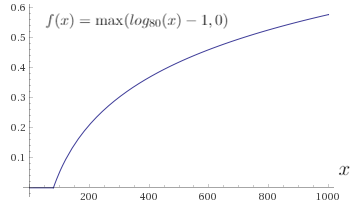
\includegraphics[width=0.55\textwidth]{resources/state_formula_plot.png}
                \caption{Example plot of the distance metric values used for track-to-detection spatial displacement cost.}
                \label{fig:state_formula_plot}
            \end{figure}
            
        \subsubsection{Appearance metric}\label{appearance_metric}
            The appearance metric is used to describe how much are the individuals visually similar, thus helps in distinguishing them. For each detected bounding box patch we calculate its appearance feature vector $r_i$ with $||r_i|| = 1$ by a forward pass of the \gls{cnn} referred in \ref{appearance_features}. Moreover, for each registered track $j$, we keep a gallery $R_j = \left\{ r_j^{(t)}\right\}_{t=1}^{L_j} $ of the last $L_j = 100$ associated appearance features. Then, the appearance distance between the $i$-th detection and the $j$-th track is defined as:
            
            \begin{equation}
                d_{c}(i,j) = \min \left\{ 1 - r_i^T r_j^{(t)} \mid  r_j^{(t)} \in R_j \right\}.
            \end{equation}
            
            The outcome of $d_c(i,j)$ is neatly bounded in $[0,1]$, where $0$ means most similar objects. This time, we introduce a threshold $t_c$ to control if an association is possible. Thus any track and detection pair with $d_c(i,j) > t_c$ is so different that it cannot be associated. For our particular scene, $t_c = 0.15$ has proved to be working well.

        \subsubsection{Matching}
           Building the associations happens in cascade fashion which is taken over from the \cite{wojke2017simple}. The cost value is based on actual state and appearance and is calculated for each possible track and detection pair. We find the best associations by running the Hungarian algorithm \cite{jonker1987shortest} that solves the min cost assignment problem. Then, we verify if the association is possible based on the appearance threshold $t_c$. If yes, we update registered tracks with associated detections. For the rest of unmatched detections, we create new tentative tracks. In Fig. \ref{fig:framework_diagram} we also provide a simplified diagram of one pass through of the algorithm cycle.
           
           \begin{figure}[ht]
                \centering
                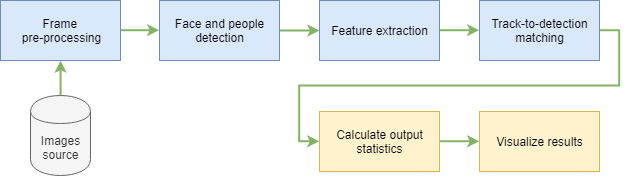
\includegraphics[width=0.75\textwidth]{resources/framework_diagram.png}
                \caption{Simplified diagram of single framework pass through. Yellow-marked boxes are optional components used for evaluation.}
                \label{fig:framework_diagram}
            \end{figure}
            
\section{Soft-biometrics extraction}
    Besides the goal of building the people detector and tracker, we also address additional information extraction related to people class -- soft-biometrics. The aim is to focus on information that can be utilized in the retail environment. Therefore we have focused on methods for estimating age, gender, emotion, height, and ground plane trajectory. Because extraction all of these features in each frame would be computationally intensive, we design our framework to be fully modular in the sense that any of the feature extractors can be turned on or off at any time.
    
    \section{Facial features}
        Before extracting any facial features, robust face detector needs to be utilized to locate faces in the image. Due to the fact the era of traditional methods such as Haar cascades \cite{viola2001rapid} is over, we decided to choose suitable face detector only from \gls{cnn}-based architectures. In particular, we designed an interface for three different \gls{cnn}-based face detectors that offer different trade-offs between speed and accuracy performance. 

        \begin{itemize}
            \item \textbf{faced} \cite{faced} is first of them achieving near real-time performance on \glsentryshort{cpu}. It uses an ensemble of two \gls{cnn}s where first is based on \gls{yolo} architecture. It takes the input image and outputs a grid where each cell contains a prediction of bounding boxes and the probability of one face. Furthermore, these outputs are fine-tuned by another custom \gls{cnn} architecture that is trained to refine bounding box coordinates. Our utilized model is pre-trained on WIDER FACE \cite{yang2016wider} dataset. 
            \item \textbf{Tensorflow Mobilenet SSD} \cite{itzcovichtfdetector} is a popular open-source face detector framework. It is based on a more robust \gls{ssd} \cite{liu2016ssd} architecture than the faced framework, thus it provides better accuracy. We utilize a pre-trained model on WIDER FACE \cite{yang2016wider} dataset that can have a real-time performance on GPU and takes only about 400 MB of \gls{gpu} memory.
            \item \textbf{MTCNN} architecture \cite{7553523} and its implementation \cite{centenomtcnn} is the last utilized face detector that achieves superior accuracy over the state-of-the-art techniques on the public datasets. It leverages a cascaded architecture with three stages of designed \gls{cnn}s to predict face and landmark location in a coarse-to-fine manner. In addition to face detection, it also performs a face alignment. The proposed architecture is a heavy, but it achieves near real-time performance on modern \gls{gpu}s. We use this architecture to compare accuracy performance with weaker face detectors.
        \end{itemize}
        
        Gathered face regions from the face detector need to be paired with people detections. This problem is solved based on the assumption that the face is in the upper middle part of the person bounding box. Face regions with confidence less than 90 \% or without associated person detection are not preserved. No additional post-processing of face regions is done in this step. With the face regions paired to people, we can finally estimate a few types of soft-biometrics.
        
        \subsection{Age and gender estimation}\label{age_gender_estimation}
            As already mentioned in \ref{age_and_gender_estimation_related}, age is most commonly estimated at the same time with gender. In this work, we built an interface for two existing \gls{cnn} models -- Keras Age and Gender \cite{kerasagender} based on \gls{dex} architecture and \gls{ssr} \cite{yang2018ssr}. However, in our specific task, the \glsentryshort{ssr} architecture with the pre-trained model provided not only more accurate predictions but better speed performance. Thus we consider only the \glsentryshort{ssr} in the final design. 
            
            Before feeding the face image patch into \gls{cnn}, we first extend the detected face region by margin $m$ as follows:
            \begin{align}
                x_{tl\textunderscore new} = \max(x_{tl\textunderscore old} - m \cdot fa_w, 0) \\
                y_{tl\textunderscore new} = \max(y_{tl\textunderscore old} - m \cdot fa_h, 0) \\
                x_{br\textunderscore new} = \max(x_{br\textunderscore old} + m \cdot fa_w, fr_w) \\
                y_{br\textunderscore new} = \max(y_{br\textunderscore old} + m \cdot fa_h, fr_h),
            \end{align}
            where $x_{tl\textunderscore new}, y_{tl\textunderscore new}$ and $x_{br\textunderscore new}, y_{br\textunderscore new}$ are new top left and bottom right coordinates of bounding box, respectively, $x_{tl\textunderscore old}, y_{tl\textunderscore old}, x_{br\textunderscore old}, y_{br\textunderscore old}$ are their corresponding original coordinates, $fa_w$ and  $fa_h$ is according width and height of face region,  $fr_w$ and $fr_h$ is according width and height of frame.
            
            If the margin $m$ is too small, then the face is not cropped entirely, and if the offsets are too big, then too much space around the face is included. Both cases affect the prediction accuracy, thus it is necessary to choose a suitable margin for a particular scene. In our case, the value margin value of $m=0.5$ worked well.
            
            Furthermore, face patches are also normalized by min-max normalization from 0 to 255 to eliminate the illumination variance:
            \begin{equation}
                    x_{norm} = \frac{( x - \min(region) ) \cdot (newmax - newmin)}{\max(region) - \min(region)} + newmin,
            \end{equation}
            where $x$ is the input pixel value, $newmin=0$, $newmax=255$, and $\min(region)$ and $\max(region)$ takes accordingly minimum or maximum value of the face region. 
            
           The output of the age classifier is a continuous value which is not further post-processed. Output values from the gender model are $x \in [0,1]$ where $x > 0.5$ means female and otherwise male. The more the value of $x$ is at the edge of the interval, the more certain the prediction is. Also, no further post-processing is needed for gender values.

        \subsection{Facial expression recognition}
            In the same spirit as the previous models, we tried to utilize at least two different architectures to estimate emotions which can be further compared. First of them is \cite{arriaga2017real} inspired by \cite{rothe2015dex} \gls{cnn} architecture, which introduces the open-source framework that can recognize seven types of face emotions -- angry, disgust, fear, happy, sad, surprise, neutral. Their model can operate in real-time, and they provide pre-trained weights on FER2013 dataset \cite{goodfellow2013challenges}. 

            Other architecture employed, known as EmoPy \cite{emopy}, is a toolkit with various \gls{cnn} architectures implemented. However, the most popular model is Fermodel which is trained to predict the same facial categories as the previously mentioned model. We decided to utilize EmoPy for the task of estimating emotions because their framework can operate with a smaller subset of all seven emotions, which is undoubtedly more practical in real-world scenarios. Furthermore, they provide more complex models that provide an output based on temporal information of past frames. The provided model can operate in real-time and is also pre-trained on FER2013 dataset \cite{goodfellow2013challenges}.
            
            For the input of EmoPy, we similarly pre-process the input face region as in \ref{age_gender_estimation}. We expand the face region by margin $m$, but we also convert the image to grayscale. This time, we do not normalize the input image, because the model was not trained in this manner. The output of the model is facial categories with their associated probabilities. We choose the most likely one and ignore the rest.
        
    \section{Spatial information}
        In addition to visual information such as facial features, we can extract additional information which relates to the spatial features of the space captured. However, these methods usually need some knowledge of the scene captured, so they cannot be applied in general. However, in our assumptions, we expected the full knowledge of the scene, thus we are not limited, and we can apply a wide range of available methods.
        
        \subsection{Trajectory}
            One of the most intuitive ways to get some spatial information in the scene is to focus on the movement in space itself. More specifically, extraction of individual's trajectories. The best way to analyze motion in space and to work with trajectories is in the top-down (or bird's eye) view. However, in most real cases of tracking people, we are unable to place the camera to achieve this kind of perspective. This placement would also prevent the possibility of obtaining further facial descriptors. Fortunately, we can transform some parts of the original image to resemble similar to a top-down view. 
            
            Formally, we can utilize 2-D projective transformation between real-world and image ground plane with its main component known as homography matrix. Since the perspective problem is considered as one of the most difficult and precise topics in \gls{cv} that goes beyond the possibilities of this work, we recommend one of the most popular books \cite{hartley2003multiple} in this field, where a detailed explanation can be found. However, if we resort to a brief explanation, then the homography matrix $H$ relates the transformation between two planes (up to a non-zero scale factor $s$) as follows:
            \begin{equation}
                s 
                \begin{pmatrix}
                    x' \\ y' \\ 1 \\
                \end{pmatrix}\
                = H
                \begin{pmatrix}
                    x \\
                    y \\
                    1 \\
                \end{pmatrix}
                =
                \begin{pmatrix}
                    h_{1,1} & h_{1,2} & h_{1,3} \\ h_{2,1} & h_{2,2} & h_{2,3} \\ h_{3,1} & h_{3,2} & h_{3,3} \\
                \end{pmatrix}
                \begin{pmatrix}
                    x \\ y \\ 1 \\
                \end{pmatrix}.
            \end{equation}
            $H$ has eight degrees of freedom, which means there are eight unknowns that need to be solved for, and it is generally normalized with $h_{3,3} = 1$ or $h_{1,1}^2 + h_{1,2}^2 + h_{1,3}^2 + h_{2,1}^2 + h_{2,2}^2 + h_{2,3}^2 + h_{3,1}^2 + h_{3,2}^2 + h_{3,3}^2 = 1$.

            Typically, an estimate of the matrix $H$ is done by finding point correspondences between the target planes. One point correspondence gives two linearly independent equations, and four correspondences are needed for a minimal solution. If more than four correspondences are known, then a more accurate solution can found according to the predefined cost function. Finally, the matrix $H$ can be estimated running \gls{dlt} algorithm \cite{hartley2003multiple}.


            There are many scenarios in \gls{cv} where a homography may be required. However, the question is how it relates to trajectories. If we have at least four ground-truth world measurements of the ground plane that are visible in the camera frame, we can build frame-to-world point correspondences and estimate the matrix $H$. Further, we can use this matrix to transform each point $(x, y)$ that lies on the ground plane in scene coordinates to real-world coordinates. For a specific example of tracking people, we assume that people are walking on a common ground plane. Thus we can take their bottom center point of the bounding box and transform it with $H$ to get the corresponding point in real-world coordinates. As a result, we can precisely estimate positions where people have walked, not in frame coordinates, but in real-world coordinates that we previously measured in the calibration phase.
            
            \begin{figure}[h]
                \centering
                \subfloat[]{{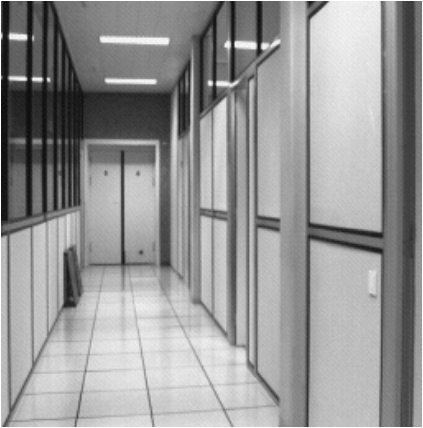
\includegraphics[width=0.25\textwidth]{resources/homograhpy_1.png} }}
                \qquad
                \subfloat[]{{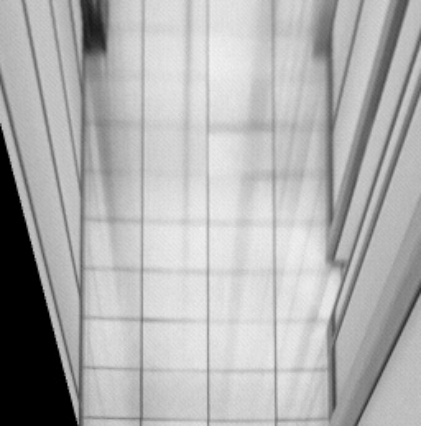
\includegraphics[width=0.25\textwidth]{resources/homography_2.png} }}
                \qquad
                \subfloat[]{{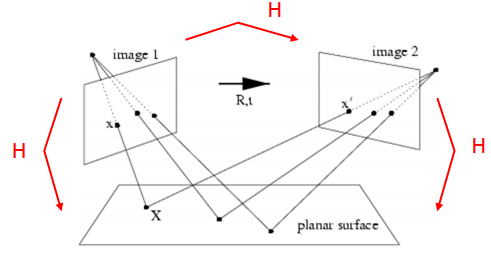
\includegraphics[width=0.35\textwidth]{resources/homography_3.png} }}
                \caption{Example of the 2-D projective transformation. a) Source image. b) Top-down view of the corridor floor generated from (a) using the four corners of a floor tile to compute the homography. c) A planar surface viewed by two camera positions is related by homography $H$, thus any point can be transformed between these different planes. Source: \cite{hartley2003multiple}}.
                \label{fig:homography_example}
            \end{figure}
  
        \subsection{Height estimation}
            In the previous section, we presented a 2-D transformation that can transform point coordinates between planes. This section deals with a related problem known as single-view metrology, which uses projective geometry to recover a structure of the 3-D world objects from a single image with several reference measurements. Since this section again contains complex theoretical concepts such as vanishing points, vanishing lines, we assume that the reader got acquainted with them from the suggested book \cite{hartley2003multiple}.
            
            Let us have a visible ground plane $p$ represented as a floor in the scene, the vanishing point $v$ in the vertical direction of the $p$, vanishing line $l$ of the $p$, $t_r$ and $b_r$ are the top and base points of the reference object, respectively and $t_x$ and $b_x$ are the top and base points of the object to be measured. All base points must lie on the $p$, and all top points must lie on a line that intersects the according to the base point and is perpendicular to $p$. Then, the $\alpha$ metric factor can be found by the following equation:
            \begin{equation}\label{height_equation_1}
                \alpha = - \frac{|| b_r \times t_r ||}{Z_r (l \cdot b_r) || v \times  t_r|| }.
            \end{equation}
            With the $\alpha$ calculated, we can estimate a height $Z_x$ for an arbitrary object that stands on the ground plane by the following equation:
            \begin{equation}\label{height_equation_2}
                  Z_x = - \frac{|| b_x \times t_x ||}{\alpha (l \cdot b_x) || v \times  t_x|| }.
            \end{equation}
            The application of this formula is most easily understood from Fig. \ref{fig:height_estimation} and the proof can be found in \cite{criminisi2002single}.
            
            To conclude, with this single-view metrology framework, we can measure the real-world height of the object that stands on the ground plane (with known $t_x$ and $b_x$ that are bounding box top or bottom point, respectively). It works for uncalibrated cameras, only real-world measurements on the ground plane and beyond are sufficient for calculating the $v$ and $l$. 

             \begin{figure}[h]
                \centering
                \subfloat[]{{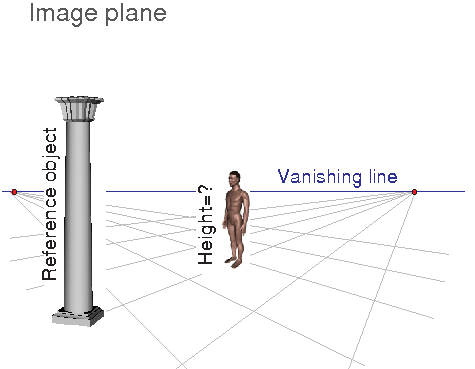
\includegraphics[width=0.4\textwidth]{resources/height_estimation_1.png} }}
                \qquad
                \subfloat[]{{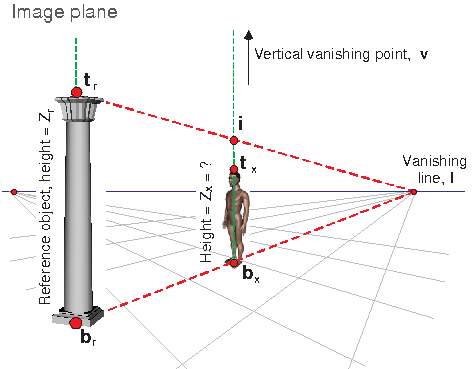
\includegraphics[width=0.4\textwidth]{resources/height_estimation_2.png} }}
                \qquad
                \subfloat[]{{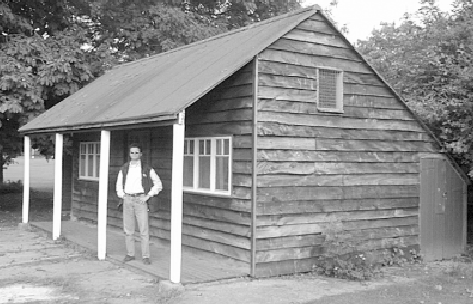
\includegraphics[width=0.4\textwidth]{resources/height_estimation_3.png} }}
                \qquad
                \subfloat[]{{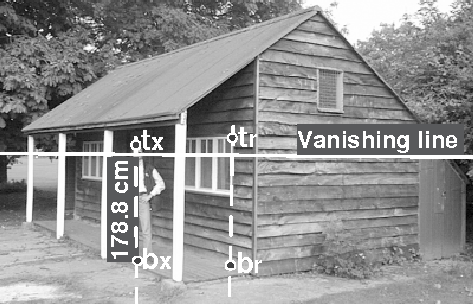
\includegraphics[width=0.4\textwidth]{resources/height_estimation_4.png} }}
                \caption{Measuring heights in single images. (a) The aim is to compute the height of the human figure relative to the height of the column (reference). The vanishing line of the ground plane has been computed and is shown blue. (b) The unknown height $Z_x$ can be computed from image quantities only as shown in \ref{height_equation_2} (c) A photograph of a garden shed in Oxford. (d) Once the height of the window top edge from the floor has been measured (reference), the height of the man is computed to be 178.8 cm which is about 1 cm off the ground truth. Source: \cite{criminisi2002single}}.
                \label{fig:height_estimation}
            \end{figure}